\section{Effiziente Berechnung der CWT}
\rhead{Berechnung der CWT}
Als erstes möchten wir herausfinden, wie sich die CWT effizient berechnen lässt.
Als zweites werden wir zwei Beispielsignale definieren und die CWT mittels Haar-Wavelet betrachten.
Abschliessend rechnen wir die CWT noch mit dem Gabor-Wavelet und vergleichen die beiden Bilder.

\subsection{CWT als Faltung}
Betrachten wir zuerst die folgende Gleichung
\begin{equation}
\Wave f (a,b)
=
\langle f,\psi_{a,b}\rangle
=
\frac{1}{\sqrt{|a|}}\int_{-\infty}^\infty f(t)\,
	\overline{\psi}\biggl(\frac{t-b}{a}\biggr)\,\mathrm{d}t,\label{complex:CWT}
\end{equation}
durch welche in Definition~\ref{cwt:definition} die kontinuierliche Wavelet-Transformation eingeführt wurde.
Dieses Integral entspricht der Faltung zwischen $f(t)$ und 
\begin{equation} 
    g(t) 
    = \frac{1}{\sqrt{|a|}} \overline\psi\biggl(\frac{-t}{a}\biggr).
\end{equation}
Der Standard-Trick zur effizienten Berechnung einer Faltung ist die Multiplikation im Frequenzbereich.
\begin{equation} 
\mathcal{W}f (a,b) = (f*g)(t) = \mathcal{F}^{-1}\biggl\lbrace\hat f(\omega) \hat g (\omega) \biggr\rbrace.
\end{equation}
Dafür benötigen wir die Fouriertransformierte $\hat g (\omega)$:
\begin{align*}
	\hat g (\omega) = 
    \Four\,\biggl\lbrace \frac{1}{\sqrt{|a|}} \overline\psi \biggl(\frac{-t}{a}\biggr) \biggr\rbrace 
	&= \frac{1}{\sqrt{|a|}} \int_{-\infty}^{\infty}\overline\psi\biggl(\frac{-t}{a}\biggr) \, e^{-i\omega t}\,\mathrm{d}t\\
	&= \frac{1}{\sqrt{|a|}} \overline{\int_{-\infty}^{\infty}\psi \biggl(\frac{-t}{a}\biggr) \, e^{i\omega t}\,\mathrm{d}t}  
    & \biggl(\text{Substitution } t' = \frac{-t}{a}\biggr)\\
	&= \frac{1}{\sqrt{|a|}} \overline{\int_{-\infty}^{\infty}\psi(t') \, e^{-ia\omega t'} |a|\,\mathrm{d}t'}\\
	&= \sqrt{|a|} \, \overline{\hat{\psi}}(a\omega).
\end{align*}
Gleichung~\eqref{complex:CWT} lässt sich somit schreiben als
\begin{equation}
\Wave f(a,b)
= \mathcal{F}^{-1}\bigl\lbrace\hat{f}(\omega) \sqrt{|a|}\, \overline{\hat{\psi}}(a\omega)\bigr\rbrace. \label{complex:fcwt}
\end{equation}

Mittels Fourier-Transformation lässt sich die Wavelet-Transformation folglich besonders elegant berechnen.
Kontinuierliche Funktionen sind für numerische Systeme jedoch ungeeignet.
Die CWT muss in $a$ und $b$ diskretisiert werden.
Die Diskretisierung von $b$ entspricht vorteilhaft gerade derjenigen des Signals selbst.
Dann lässt sich die Fourier-Transformation mittels FFT effizient berechnen und Gleichung~\eqref{complex:fcwt} wird zu
\begin{equation}
	\mathcal{W}f(a,b) = \text{IFFT}\bigl(\text{FFT}(f) \, \overline{\hat{\psi}}(a\omega)\bigr). \label{complex:ffcwt}
\end{equation}

Der Faktor $\sqrt{|a|}$ wurde hierbei weggelassen.
Hierdurch werden die hohen Frequenzen stärker gewichtet und $|\!\Wave f(a,b)|$ ist gerade proportional zur Amplitude der analysierten Signalkomponente.
Zudem erzielen wir im Diskreten nicht exakt die Faltung, sondern die zirkuläre Version davon. 
Mehr dazu im Abschnitt~\ref{complex:circ-conv-padding}.

Gleichung~\eqref{complex:ffcwt} muss für jedes $a$ einzeln gelöst werden.
Sie wird besonders interessant, wenn das Wavelet im Frequenzbereich eine geschlossene, analytische Form besitzt.
Dann benötigt man nur eine FFT für das Signal, so wie für jedes $a$ eine inverse FFT und eine punktweise Multiplikation zwischen Signal und Wavelet.

\clearpage
\subsection{Das Haar-Wavelet}
\rhead{Haar-Wavelet}
\begin{figure}
	\centering
	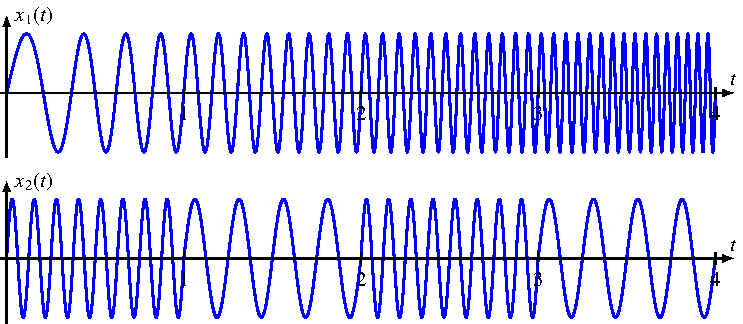
\includegraphics{papers/complex/images/signals.pdf}
	\caption{Die beiden Beispielsignale $x_1(t)$ und $x_2(t)$}
\end{figure}
Rechnen wir das erste Beispiel.
Hierfür benötigen wir zwei Dinge: Signal und Wavelet.
Als Signale nehmen wir zwei Sinus-Schwingungen, eine mit linear ansteigender und eine mit stückweise konstanter Frequenz.
\begin{align}
    x_1(t) &= \sin\left( \int_{0}^{t} 2\pi f_1(t')\,\mathrm{d}t'\right) & f_1(t) &= 2 + 6/4 \cdot t \\
    x_2(t) &= \sin\left( \int_{0}^{t} 2\pi f_2(t')\,\mathrm{d}t'\right) & f_2(t) &= \left\lbrace \begin{matrix}
    4, & &t& < 1\\
    8, & 1.0 \le &t& < 2.0\\
    4, & 2.0 \le &t& < 3.0\\
    8, & 3.0 \le &t&\\
    \end{matrix}\right.
\end{align}
Das Haar-Wavelet sei in diesem Abschnitt zentriert um $t=0$.
Die daraus resultierende Symmetrie wird sich in der Berechnung der Fourier-Transformation als hilfreich erweisen.

\begin{definition}
	\label{complex:def-haar-wavelet}
	Das Haar-Wavelet besitzt folgende Gestalt:
	\[
	\psi_{\text{Haar}}(t) = \left\lbrace\begin{matrix*}[r]
	1 & -\frac{1}{2} \le t < 0  \\
	-1 & 0 \le t < \frac{1}{2} \\
	0 & \text{sonst}.
	\end{matrix*} \right.\label{complex:def-haar}
	\]
\end{definition}
Die Fourier-Transformierte von $\psi_{\text{Haar}}$ berechnet sich wie folgt:
\begin{align}
	\Four \psi_\text{Haar}  
	&= \frac{1}{\sqrt{2\pi}}\int_{-\infty}^{\infty} \psi_\text{Haar} e^{-i\omega t} \,\mathrm{d}t\nonumber\\
	&= \frac{1}{\sqrt{2\pi}}\Biggl( \int_{-1/2}^{0} e^{-i\omega t} \,\mathrm{d}t - \int_{0}^{1/2} e^{-i\omega t}\,\mathrm{d}t \Biggr) \nonumber\\
	&= \frac{i}{\sqrt{2\pi}\omega}\bigl( \bigl[ e^{-i\omega t}\bigr]_{-1/2}^0  - \bigl[ e^{-i\omega t}\bigr]_{0}^{1/2} \bigr)\nonumber\\
	&= \frac{i}{\sqrt{2\pi}} \frac{1-\cos(\omega/2)}{\omega/2}\label{complex:f-psi-haar}
\end{align}
Das Haar-Wavelet ist also nicht nur im Zeitbereich besonder einfach, sondern auch im Frequenzbereich.
Insbesondere lässt sich die mit $a$ skalierte Version des Wavelets durch Satz~\ref{four-int:trans-dial} direkt im Frequenzbereich berechnen.
Abbildung~\ref{complex:haar} zeigt das Haar-Wavelet im Zeit- und Frequenzbereich.
Auffallend ist, dass das im Zeitbereich besonders gut lokalisierte Haar-Wavelet in der Frequenz sehr schlecht lokalisiert ist.
\begin{figure}
	\centering
	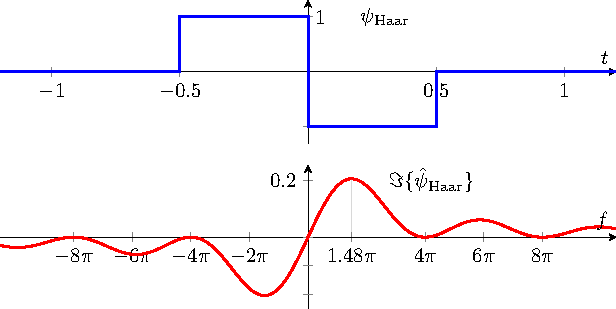
\includegraphics{papers/complex/images/haar.pdf}
	\caption{Das Haar-Wavelet}
	\label{complex:haar}
\end{figure}

\begin{figure}
	\centering
	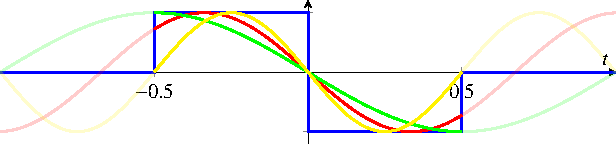
\includegraphics{papers/complex/images/haar_dom.pdf}
	
	\caption{Blau: $\psi_\text{Haar}$, Rot: $\sin ({\color{red}\omega_\psi}\cdot t)$, Gelb: $\sin ({\color{yellow}1.0}\cdot 2\pi t)$, Grün: $\sin ({\color{green}0.5}\cdot 2\pi t)$}
	\label{complex:dom-freq}
\end{figure}
An dieser Stelle definieren wir noch die \emph{dominante Frequenz} eines Wavelets.
\begin{definition}
	Die Fourier-Transformierte eines Wavelets erreicht den maximalen Betrag bei der \emph{dominante Frequenz $\omega_\psi$}.
	\begin{equation}
		\omega_\psi \coloneqq \underset{\omega}{\text{\emph{argmax}}} \, |\hat\psi(\omega)|
	\end{equation}
	
\end{definition}

Die dominante Frequenz erlaubt es, die $a$-Achse der Wavelet-Transformation als Frequenz-Achse zu interpretieren.
Für die Momentanfrequenz gilt
\[
	\omega(b) \approx \frac{\omega_\psi}{a_\text{max}(b)},
	\quad 
	a_\text{max}(b)
	= 
	\underset{a}{\text{argmax}} \, |\!\Wave f(a,b)|.
\]
Diese Interpretation ist natürlich nur zulässig, wenn das Signal zum betrachteten Zeitpunkt nur eine dominante Frequenz-Komponente beinhaltet.
Bei unseren Beispielsignalen ist dies der Fall.
Abbildung~\ref{complex:dom-freq} illustriert die Bedeutung von $\omega_\psi$ für das Haar-Wavelet.
Es ist die Frequenz, bei welcher das Skalarprodukt mit dem Wavelet maximal wird.

Somit haben wir für unser Beispiel alles zusammen.
Nach einer Diskretisierung der Variablen überlassen wir die Arbeit dem Computer.
Dies liefert die Bilder aus Abbildung~\ref{complex:haar-ex}.

\begin{figure}
	\centering
	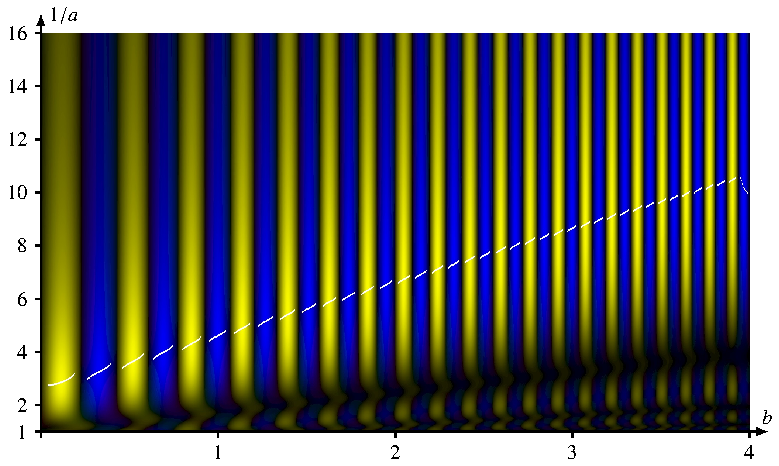
\includegraphics{papers/complex/images/chirp_haar.pdf}
	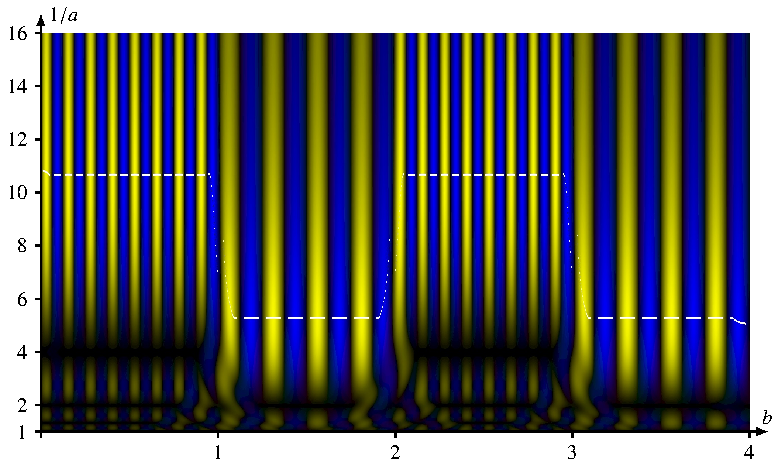
\includegraphics{papers/complex/images/square_haar.pdf}
	\caption{Wavelet-Transformationen der beiden Beispielsignale mit dem Haar-Wavelet. Die Lokalisierung in der Zeit ist sehr gut, aber die momentane Frequenz ist ohne Weiteres kaum ersichtlich. Zudem resultiert das periodische Signal in einer periodischen Helligkeit. (Zur Erinnerung: Blau entspricht $+1$, Gelb entspricht $-1$)}
	\label{complex:haar-ex}
\end{figure}

Wie erwartet ist die Lokalisierung in der Frequenz zimelich schlecht.
Das Haar-Wavelet gibt den Zeitpunkt einer Änderungen der Frequenz zwar sehr genau wieder, die Frequenz selbst ist jedoch kaum ablesbar.
Als Orientierungshilfe sind $a_\text{max} (b) = \max_a{|\!\Wave x_n(a,b)|}$ weiss hervorgehoben.
Sie weichen um $\omega_\psi$ von der Signal-Frequenz ab, welche als Schwingung in der Amplitude gut erkennbar ist.
Dieses An- und Abschwellen des Betrags der Skalarprodukte verhindert es, $a_\text{max}(b)$ einfach zu folgen.
Dies werden wir im Abschnitt~\ref{complex:separate} durch komplexe Wavelets beheben.
Zuerst kümmern wir uns aber um die Lokalisierung in der Frequenz.
